\let\negmedspace\undefined
\let\negthickspace\undefined
\documentclass[journal,12pt,onecolumn]{IEEEtran}
\usepackage{cite}
\usepackage{amsmath,amssymb,amsfonts,amsthm}
\usepackage{algorithmic}
\usepackage{graphicx}
\usepackage{textcomp}
\usepackage{xcolor}
\usepackage{txfonts}
\usepackage{listings}
\usepackage{enumitem}
\usepackage{mathtools}
\usepackage{gensymb}
\usepackage{comment}
\usepackage{caption}
\usepackage[breaklinks=true]{hyperref}
\usepackage{tkz-euclide} 
\usepackage{listings}

\usepackage{gvv}                                        
%\def\inputGnumericTable{}                                 
\usepackage[latin1]{inputenc}     
\usepackage{xparse}
\usepackage{color}                                            
\usepackage{array}                                            
\usepackage{longtable}                                       
\usepackage{calc}                                             
\usepackage{multirow}
\usepackage{multicol}
\usepackage{hhline}                                           
\usepackage{ifthen}                                           
\usepackage{lscape}
\usepackage{tabularx}
\usepackage{array}
\usepackage{float}
%\newtheorem{theorem}{Theorem}[section]
%\newtheorem{theorem}{Theorem}[section]
%\newtheorem{problem}{Problem}
%\newtheorem{proposition}{Proposition}[section]
%\newtheorem{lemma}{Lemma}[section]
%\newtheorem{corollary}[theorem]{Corollary}
%\newtheorem{example}{Example}[section]
%\newtheorem{definition}[problem]{Definition}

\begin{document}

\title{8.3.15}
\author{AI25BTECH11035 - SUJAL RAJANI}
% \maketitle
% \newpage
% \bigskip
%\begin{document}
{\let\newpage\relax\maketitle}
%\renewcommand{\thefigure}{\theenumi}
%\renewcommand{\thetable}{\theenumi}
% \newpage
% \bigskip
\textbf{QUESTION}
An equilateral triangle is inscribed in the parabola $y^2=4ax$
, where one vertex is at the vertex of the parabola . Find the length of the side of the triangle .
\\
\textbf{SOLUTION}
 let the three position vector  of the equilateral triangle be $\vec{A}$,$\vec{B}$ and $\vec{C}$ .
 \\
 let 
 \\
 \begin{align*}
     \vec{A}=\myvec{0\\0}, \vec{B}=\myvec{x\\y}, \vec{C}=\myvec{x\\-y}
 \end{align*}
 both parabola and equilateral triangle are symmetric about x axis  that why the y coordinates of $\vec{B} $and $\vec{C}$ are of different sign .
 \\
  \begin{align*}
      y^2=4ax 
  \end{align*}
  because the position vector of $\vec{B}$ and $\vec{C}$ lie of the parabola .
  \begin{align*}
      ||\vec{B}-\vec{A}||^2=||\vec{B}-\vec{C}||^2
      \\
      (\vec{B}-\vec{A})^\top(\vec{B}-\vec{A})=(\vec{B}-\vec{C})^\top(\vec{B}-\vec{C}) .
      \\
      y^2+x^2=4y^2
      \\
      x=12a.
 \end{align*}
 by replacing the value of x in (1) equation :
\\
\begin{align*}
    y^2=48a^2
    \\
    y=\sqrt{48}a
\end{align*}
the length of side of equilateral triangle is :
\begin{align*}
    2y=2\sqrt{48}a.
\end{align*}
        \begin{figure}[H]
    \centering
    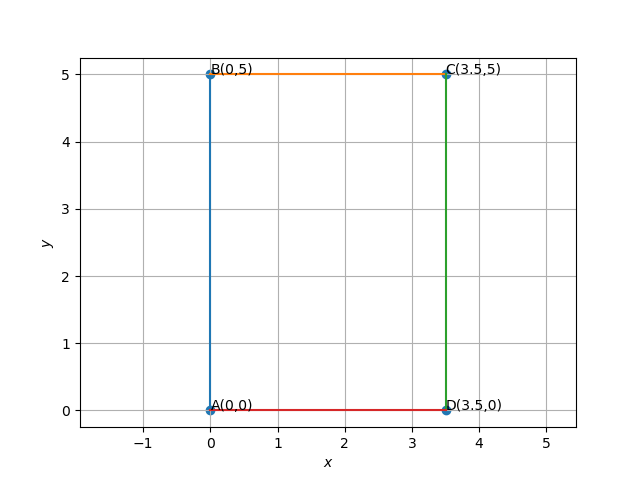
\includegraphics[width = 0.7\columnwidth]{../figs/img.png}
    \caption*{}
    \label{figs}
\end{figure}

\end{document}